\documentclass[12pt, letterpaper]{article}

\usepackage[margin=1in]{geometry}
\usepackage[margin=0.5in]{caption}

\usepackage{aliascnt}
\usepackage{amsmath}
\usepackage{amsthm}
\usepackage{amssymb}
\usepackage[backend=bibtex]{biblatex}
\usepackage[noabbrev,capitalize,nameinlink]{cleveref}
\usepackage{graphicx}
\usepackage{mathtools}
\usepackage{microtype}
\usepackage{tikz}

\usetikzlibrary{arrows,arrows.meta,automata,calc, positioning}

\newcommand{\paren}[1]{\left(#1\right)}
\newcommand{\pfrac}[2]{\paren{\frac{#1}{#2}}}

\newcommand{\Z}{\mathbb Z}
\newcommand{\N}{\mathbb N}
\newcommand{\Q}{\mathbb Q}
\newcommand{\C}{\mathbb C}
\newcommand{\bin}{\mathbf 2}
\newcommand{\A}{\mathcal A}
\newcommand{\CC}{\mathsf{CC}}
\newcommand{\ch}[1]{\mathbf{#1}}
\newcommand{\res}[2]{{{#1}_{\ch{#2}}}}
\newcommand{\I}{\mathcal I}
\renewcommand{\S}{\mathcal S}
\newcommand{\comp}{\mathfrak C}
\newcommand{\princ}{\mathfrak A}
\newcommand{\Aut}{\mathbf{Aut}}
\newcommand{\sg}{\mathcal S}
\newcommand{\gp}{\mathcal G}
\newcommand{\set}[1]{\left\{#1\right\}}
\newcommand{\R}{\mathbf R}
\newcommand{\f}[1]{\overline{#1}}
\newcommand{\ideal}{\mathfrak{I}}
\newcommand{\disc}[1]{\text{Disc}\paren{#1}}
\newcommand{\orb}{\mathbf{orb}}
\newcommand{\rk}[1]{\left|#1\right|}

\newcommand{\codeurl}{\texttt{https://github.com/tim-becker/thesis-code}}

\bibliography{thesis}

\newtheorem{thm}{Theorem}[section]
\newtheorem{lemma}[thm]{Lemma}
\newtheorem{cor}[thm]{Corollary}
\newtheorem{defn}[thm]{Definition}
\newtheorem{prop}[thm]{Proposition}
\newtheorem{conj}[thm]{Conjecture}
\newtheorem{example}[thm]{Example}
\crefname{thm}{Theorem}{Theorems}
\crefname{lemma}{Lemma}{Lemmas}
\crefname{cor}{Corollary}{Corollaries}
\crefname{defn}{Definition}{Definitions}
\crefname{conj}{Conjecture}{Conjectures}
\crefname{prop}{Proposition}{Propositions}
\crefname{example}{Example}{Examples}

\tikzset{%
        ->,
        auto,
        shorten > = 2pt,
        node distance=2.5cm
}
\tikzstyle{every state}=[
    draw = black,
    style = thick,
    fill = white,
    line width = 1pt,
    minimum size = 5mm
]
\tikzstyle{every edge}=[
    style = thick,
    draw = black,
    line width=1pt,
]


\title{Orbits of Abelian Automaton Groups}
\author{Tim Becker\\ \texttt{tbecker@cs.wisc.edu}\\\\
        Klaus Sutner\\ \texttt{sutner@cs.cmu.edu}}
\date{}
\begin{document}

\maketitle

\abstract{%
    Automaton groups are a class of groups generated by invertible finite-state
    transducers. We study properties of abelian automaton groups and their
    applications to the complexity of computational problems arising within
    these groups. We demonstrate a correspondence between abelian automaton
    groups and a class of ideals of a corresponding algebraic number field.
    Properties of this number field are utilized to construct efficient
    algorithms for problems related to orbits of finite state transductions.
    The algorithms developed within are implemented in the SageMath computer
    algebra system and are publicly available.
}


\section{Introduction}
An \emph{invertible binary transducer} $\A$ is a Mealy automaton over the
binary alphabet where each state has an invertible output function. The
transductions of $\A$ are therefore length-preserving invertible functions on
binary strings. These transductions (along with their inverses) naturally
generate a group under composition, denoted $\gp(\A)$. Such groups, over a
general alphabet, are called automaton groups or self-similar groups; these
groups have been studied in great detail, see \cite{nekrashevych2014self,
    grigorchuk2000automata} for extensive studies.

Automaton groups have many interesting properties and are capable of surprising
complexity. A number of well-known groups can be generated by fairly simple
transducers, indicating that transducers may be a useful semantic
interpretation for many groups. Bartholdi's recent book review in the Bulletin
of the AMS about the relationship between syntactic and semantic approaches to
algebra gives some examples where transducers play such a role
\cite{Bartholdi17:syntax_semantic_review}.  For instance, after Grigorchuk
famously solved the long-open problem of finding a group of intermediate
growth, it was realized that his group can be generated by the 5-state
invertible binary transducer shown in \cref{fig:grigorchuk}.  In fact, even
3-state invertible binary transducers generate groups which are exceedingly
complicated, see \cite{2008arXiv0803.3555B} for a classification of all such
automata.
\begin{figure}[ht]
    \centering
    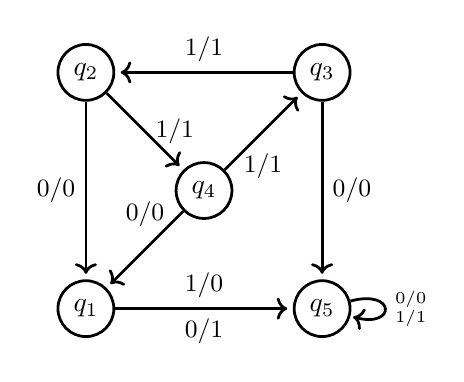
\begin{tikzpicture}[node distance=3cm]
        \node[state] (1) {$q_1$};
        \node[state] (2) [above of=1] {$q_2$};
        \node[state] (3) [right of=2] {$q_3$};
        \node[state] (4) at ($(1)!0.5!(3)$) {$q_4$};
        \node[state] (5) [right of=1] {$q_5$};
      \path
      (1)
      edge node{\small $1/0$} node[swap]{\small $0/1$} (5)
      (2)
      edge node[left]{\small $0/0$} (1)
      edge node[right]{\small $1/1$} (4)
      (4)
      edge node[above=0.15]{\small $0/0$} (1)
      edge node[below=0.15]{\small $1/1$} (3)
      (3)
      edge node[above]{\small $1/1$}  (2)
      edge node[right]{\small $0/0$}  (5)
      (5)
      edge[loop right=45] node{\small $\substack{0/0\\1/1}$} (5)
      ;
    \end{tikzpicture}
    \caption{An invertible binary transducer generating Grigorchuk's group}
    \label{fig:grigorchuk}
\end{figure}

Here, we will be primarily concerned with a simpler class of transducers: those
which generate abelian groups. This situation has been previously studied in
\cite{Okano-Thesis, Sutner18:abelian_automata}. It is known that all abelian
automaton groups are either boolean or free abelian \cite{Okano-Thesis}, and in
the free abelian case, one can show that the underlying automata have nice
structural properties. We will summarize and build upon these results in
\cref{sec:abelian-automata}.  A running example in this paper will be the
transducer $\CC^3_2$, shown in \cref{fig:cc-3-2}. This transducer generates a
group isomorphic to $\Z^2$ and is perhaps the simplest nontrivial transducer
generating an abelian group.


We will make connections between abelian automaton groups and other areas of
algebra that will provide useful insight into their structure and complexity.
A result of Nekrashevych and Sidki shows that the groups admit embeddings
into $\Z^m$ where transitions in the transducer correspond to affine maps
\cite{nekrashevych2004automorphisms}.  In this paper, we describe a related
embedding of abelian automaton groups into associated algebraic number fields
and describe how these may be efficiently computed.

Properties of this embedding can be used to study computational problems
arising in automaton groups. Given a transduction $f \in \gp(\A)$, we write
$f^* \subseteq \bin^* \times \bin^*$ for the transitive closure of $f$.  Note
that $f^*$ is a length-preserving equivalence relation on $\bin^*$.  The
complexity of this relation was first studied in \cite{jalc170214}, where it
was shown that for a certain class of abelian transductions $f$, $f^*$ is
rational. We will refer to such transductions as \emph{orbit-rational}. For
instance, it was shown in \cite{jalc170214} that $\CC^3_2$ is orbit-rational.
In this paper, we answer a more general question by giving a precise
characterization of orbit-rational abelian transducers and a corresponding
decision procedure.

Throughout this paper, we will utilize the theory of free abelian groups,
linear algebra, field theory, and some algebraic number theory. See
\cite{Hungerford78} for the necessary material on the latter subjects, and
\cite{ireland1990classical, stein2012algebraic} for background on algebraic
number theory.
\begin{figure}[hb]
    \centering
    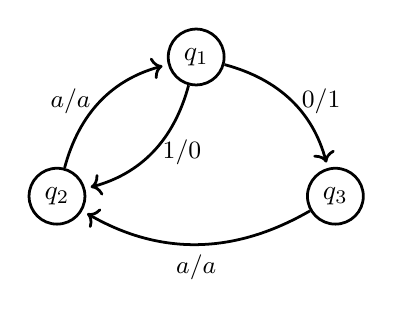
\begin{tikzpicture}
        \node[state] (1) {$q_1$};
        \node[state] (2) [below left of = 1] {$q_2$};
        \node[state] (3) [below right of = 1] {$q_3$};
        \path
        (1) edge[bend left, right]
        node {\small $1/0$} (2)
        (1) edge[bend left, right]
        node {\small $0/1$} (3)
        (2) edge[bend left, left]
        node {\small $a/a$} (1)
        (3) edge[bend left]
        node {\small $a/a$} (2)
        ;
    \end{tikzpicture}
    \caption{The cycle-cum-chord transducer $\CC^3_2$}
    \label{fig:cc-3-2}
\end{figure}

\section{Background}
\subsection{Automata and Automaton Groups}
A \emph{binary transducer} is a Mealy automaton of the form $\A = \langle Q,
\bin, \delta, \lambda \rangle$ where $Q$ is a finite state set, $\delta: Q
\times \bin \rightarrow Q$ is the transition function, and $\lambda: Q \times
\bin \rightarrow \bin$ is the output function. Such a machine is
\emph{invertible} if for each state $q \in Q$, the output function $\lambda(q,
\cdot)$ is a permutation of $\bin$. A state $q$ is called a \emph{toggle} state
if $\lambda(q, \cdot)$ is the transposition and a \emph{copy} state otherwise.
We define the transduction of $q$, $\underline{q}: \bin^* \rightarrow \bin^*$
recursively as follows: $\underline{q}(\epsilon) = \epsilon$ and
$\underline{q}(a \cdot w) = \lambda(q, a) \cdot \underline{\delta(q, a)}(w)$,
where $\epsilon$ denotes the empty string, $\cdot$ denotes concatenation, and
$a \in \bin$. Note that invertibility of transductions follows from
invertibility of the transition functions.  The inverse machine $\A^{-1}$ is
computed by simply flipping the edge labels of $\A$: if
$p \xrightarrow{\ch{a} / \ch{b}} q$ in $\A$ then
$p^{-1} \xrightarrow{\ch{b} / \ch{a}} q^{-1}$ in $\A^{-1}$.

Invertible transducers define a subclass of automaton groups. The group
$\gp(\A)$ is formed by taking all transductions and their inverses under
composition.  As described in \cite{jalc170214} the group $\gp(\A)$ can be seen
as a subgroup of the automorphism group of the infinite binary tree, denoted
$\Aut(\bin^*)$.  Clearly any automorphism $f \in \Aut(\bin^*)$ can be written
in the form $f = (\res{f}{0}, \res{f}{1})\pi$ where $\pi \in S_2$. Here $\pi$
describes the action of $f$ on the root, and $\res{f}{0}$ and $\res{f}{1}$ are
the automorphisms induced by $f$ on the two subtrees. We call $(\res{f}{0},
\res{f}{1})\pi$ the \emph{wreath representation} of $f$; this name is derived
from the fact that $\Aut(\bin^*) \cong \Aut(\bin^*) \, \wr \, S_2$, where $\wr$
denotes the wreath product. Let $\sigma \in S_2$ denote the transposition. A
transduction $f$ is called \emph{odd} if $f = (\res{f}{0}, \res{f}{1}) \sigma$
and \emph{even} otherwise. In the even case, we'll write $f = (\res{f}{0},
\res{f}{1})$. We call the maps $f \mapsto \res{f}{a}$ for $\ch{a} \in \bin$ the
\emph{residuation maps}. Residuals can be extended to arbitrary length words by
$\res{f}{\epsilon} = f$ and $\res{f}{w \cdot a} = \res{(\res{f}{w})}{a}$, where
$w \in \bin^*$ and $a \in \bin$. The complete group automaton for $\A$, denoted
$\comp(\A)$, has as its state set $\gp(\A)$ with transitions of the form $f
\xrightarrow{\ch{a} / \ch{b}} \res{f}{a}$, where $\ch{b} = f \ch{a}$.

\subsection{Abelian Automata} \label{sec:abelian-automata}
For any automorphism $f \in \gp(\A)$, define its gap to be $\gamma_f =
(\res{f}{0})(\res{f}{1})^{-1}$, so that $\res{f}{0} = \gamma_f \res{f}{1}$. An
easy induction on the wreath product shows the following \cite{Okano-Thesis}:
\begin{lemma}\label{lemma:gap}
    An automaton group $\gp(\A)$ is abelian if, and only if, all even elements
    of G have gap value $I$, where $I$ denotes the identity automorphism, and
    all odd elements have the same gap.
\end{lemma}
Thus, for abelian groups, we may denote the shared gap value by $\gamma_\A$,
and when the underlying automaton is clear from context, we will simply denote
the gap value by $\gamma$.  It follows that every odd $f$ satisfies $f =
(\gamma \res{f}{1}, \res{f}{1})\sigma$ and every even $f$ satisfies $f =
(\res{f}{1}, \res{f}{1})$.

If $\gp(\A)$ is abelian, we will call $\A$ an \emph{abelian automaton}. It
should be noted that \cref{lemma:gap} gives an easy decision procedure to
determine if a given machine $\A$ is abelian. Let $\mathcal B$ be the
minimization of the product machine $\A \times \A^{-1}$, which can be computed
using a partition-refinement algorithm, where the initial partition is induced
by even and odd states. Then $\A$ is abelian if and only if the gap of each
even state is collapsed to the identity state in $\mathcal B$ and if the gap of
each odd state is collapsed to the same state in $\mathcal B$.

\section{Affine Residuation Parametrization}\label{sec:alg-num-theory}
In this section we will discuss embeddings of abelian automaton groups where
residuation corresponds to an affine map.

\subsection{Residuation Pairs}\label{sec:matrix_rep}
When $\gp(\A) \cong \Z^m$, elements of the group may be represented as integer
vectors in $\Z^m$. This section will use this interpretation, and explore the
linear-algebraic properties of the residuation maps.  Let $H \le \gp(\A)$ be
the subgroup of even automorphisms. It's clear that $H$ is a subgroup of index
2 and that the residuation maps restricted to $H$ are homomorphisms into
$\gp(\A)$. Maps of this form are known as 1/2-endomorphisms and were studied by
Nekrashevych and Sidki in \cite{nekrashevych2004automorphisms}. The authors
proved that when $\gp(\A)$ is free abelian, the residuation maps take the form
of an affine map.
\begin{thm}\label{thm:nekrashevych_sidki}
    If $\gp(\A) \cong \Z^m$, then there exists an isomorphism $\phi : \gp(\A)
    \rightarrow \Z^m$, an $m \times m$ rational matrix $A$, and a rational
    vector $r$ which satisfy
    \begin{equation}\label{eq:Aresiduals}
        \phi(\res{f}{a}) = \begin{cases}
            A \cdot \phi(f) & \text{if $f$ is even,}\\
            A \cdot \phi(f) + (-1)^a r &
            \text{if $f$ is odd.}\\
        \end{cases}
    \end{equation}
    Also, the matrix $A$ satisfies several interesting properties:
    \begin{itemize}
        \item $A$ is contracting, i.e., its spectral radius is less than 1.
        \item The characteristic polynomial $\chi(z)$ of $A$ is irreducible
            over $\Q$, and has the form $\chi(z) = z^m + \frac{1}{2}g(z)$,
            where $g(z) \in \Z[z]$ is of degree at most $m-1$.
    \end{itemize}
\end{thm}\hfill\\
We'll call the pair $A, r$ a \emph{residuation pair} for $\A$.  Then $\gp(\A)$
(and its residuation relations) is completely determined by the image of one
state under $\phi$ and a residuation pair.

\begin{example}
    $\CC^3_2$ admits the following resiudation pair:
    \begin{align*}
        A = \begin{pmatrix}
            -1 & 1\\
            -1/2 & 0
        \end{pmatrix}
        &&
        r = \begin{pmatrix}-1\\-3/2\end{pmatrix}
        &&
        \phi(s_1) = \begin{pmatrix} 1\\0 \end{pmatrix}
    \end{align*}
    The image of other states may be obtained by residuation:
    \begin{align*}
        \phi(s_2) = A \phi(s_1) - r = \begin{pmatrix}
            0\\
            1
        \end{pmatrix}
        &&
        \phi(s_3) = A \phi(s_1) + r = \begin{pmatrix}
            -2\\
            -2
        \end{pmatrix}
    \end{align*}
\end{example}

This parameterization is a useful tool for performing computations in
$\gp(\A)$. Transduction composition becomes vector addition and residuation
becomes an affine map over $\Z^m$.  However, the residuation pair is not
unique. In fact, the matrix $A$ may not be unique even up to $GL(m, \Z)$
similarity.  A theorem of Latimer and MacDuffee implies that the $GL(m, \Z)$
similarity classes of matrices with characteristic polynomial $\chi_A(z)$ are
in one-to-one correspondence with the ideal classes of $\Z[z]/(\chi_A(z))$
\cite{latimer-macduffee}.  Utilizing computer algebra, we can find an example
with multiple similarity classes.
\begin{example}
    The residuation matrices of the automaton $\CC^{15}_8$ have $2$ $GL(m, \Z)$
    similarity classes.
\end{example}

Furthermore, it is unclear at this point how one may compute a residuation pair
for a general abelian automaton.

\subsection{Number Field Embedding}\label{sec:field-rep}
We introduce a parametrization which addresses the above concerns, i.e.\ it
will be unique for $\A$, and we will give a method to compute it efficiently.
We will show that $\gp(\A)$ can be embedded as an additive subgroup of an
algebraic number field $F(\A)$. At this point, it is not clear that $F(\A)$ is
unique, but this will indeed be the case, as shown in
\cref{thm:field_representation_unique}.  In this section, we will use some
basic results from algebraic number theory, see \cite{ireland1990classical,
stein2012algebraic} for the requisite background.

Suppose $\A$ has states $q_1, \ldots, q_n$. For each state $q_i$, we introduce
an unknown $x_i$, and let $R = \Q[z, x_1, \ldots, x_n]$. For each transition
$q_i \xrightarrow{c} q_j$ in $\A$, we define the polynomial
$p_{i,j} \in R$ as $p_{i,j} = z x_i - x_j + c$. Let $\I$ be the ideal of $R$
generated by the set of all such polynomials, and let $\S$ be the system of
equations defined by $\I$, i.e.\ by setting each $p_{i,j} = 0$.

\begin{lemma}\label{lemma:solution_exists}
    The polynomial system $\S$ has a solution.
    \begin{proof}
        Let $A, r$ be a residuation pair of $\A$ and let $\chi(z)$ be the
        characteristic polynomial of $A$. Define $F = \Q(\alpha)$, where
        $\alpha$ is any root of $\chi(z)$, and let $\phi : \gp(\A) \rightarrow
        \Z^m$ be the isomorphism from \cref{thm:nekrashevych_sidki}. We will
        construct a map $\psi: \Z^m \rightarrow F$ such that applying $\psi
        \circ \phi$ to the states of $\A$ yields a solution to $\S$.

        Since $\chi(z)$ is irreducible, it's clear that $\mathcal B = \{r, Ar,
        \ldots, A^{m-1}r\}$ is a basis for $\Q^m$.  Define $\psi : \Q^m
        \rightarrow F$ on $\mathcal B$ as $\psi(A^k r) = \alpha^k$.  Then we
        have an injective homomorphism $\Psi: \gp(\A) \rightarrow F$, where
        $\Psi = \psi \circ \phi$.  Now applying $\psi$ to the terms in
        \cref{eq:Aresiduals} gives
        \begin{equation}
            \label{eq:aresiduals} \Psi(\res{f}{a}) = \begin{cases}
                \alpha \Psi(f) & \text{if $f$ is even,}\\
                \alpha \Psi(f) + (-1)^a & \text{if $f$ is odd.}
            \end{cases}
        \end{equation}
        It follows that $\alpha, \Psi(q_1), \ldots, \Psi(q_n)$ is a solution to
        $\S$.
    \end{proof}
\end{lemma}


We now analyze the structure of a general solution to $\S$, and show that up to
conjugates, the above solution is unique. For an example of such a solution,
look forward to \cref{example:field-cc-3-2}.  For the following results, let
$\alpha$, $\beta_1, \ldots, \beta_n \in \C$ be solutions for $z, x_1, \ldots,
x_n$ respectively. Define the map $\Psi$ on the generators of $\gp(\A)$ as
$\Psi(q_i) = \beta_i$.

\begin{lemma}\label{lemma:residuation}
    For each $f \in \gp(\A)$, \cref{eq:aresiduals} holds.
    \begin{proof}
        The definition of the generators of $\I$ ensures that it holds for the
        generators of $\gp(\A)$. This can be extended to arbitrary products by
        induction on the length of the product. Let $f \in \gp(\A)$, and write
        $f = s \cdot g$, where $s$ is a generator and $g \ne I$. By induction
        we have that both $s$ and $g$ obey \cref{eq:aresiduals}.  Consider the
        possible parities of $s$ and $g$; if both are even, then we have
        \[
            \alpha \Psi(f) =
            \alpha (\Psi(s) + \Psi(g)) =
            \alpha \Psi(s) + \alpha \Psi(g) =
            \Psi(\res{s}{a}) + \Psi(\res{g}{a}) = \Psi(\res{f}{a}).
        \]
        Likewise, if $s$ is odd and $g$ is even, then note $\alpha \Psi(s) =
        \Psi(\res{s}{a}) - {(-1)}^a$, and so
        \begin{align*}
            \alpha \Psi(f) + {(-1)}^a =
            \alpha \Psi(s) + \alpha \Psi(g) + {(-1)}^a =
            \Psi(\res{s}{a}) + \Psi(\res{g}{\f{a}}) =
            \Psi(\res{f}{a}).
        \end{align*}
        The final case follows similarly.
    \end{proof}
\end{lemma}


\begin{lemma}\label{lemma:a_unique}
    $\alpha$ is unique up to conjugates, i.e.\ it is a root of $\chi(z)$, the
    characteristic polynomial of a residuation matrix of $\A$.
    \begin{proof}
        Let $\gamma$ be the gap value for $\A$ discussed in
        \cref{sec:matrix_rep}. From \cref{lemma:residuation}, we see
        $\Psi(\gamma) = 2$. Let $m$ be the rank of $\gp(\A)$, and let
        $\zeta_k$ be a non-identity length-$k$ residual of $\gamma$, so that
        for $k = 1, \ldots, m$, $\Psi(\zeta_i)$ is a polynomial in $\alpha$ of
        degree $k$. Then $\gamma, \zeta_1, \ldots, \zeta_{m}$ are linearly
        dependent in $\gp(\A)$, and hence are also under $\Psi$. This shows
        that $\alpha$ is a root of a degree $m$ polynomial, which is the the
        same degree as the irreducible $\chi(z)$ from
        \cref{lemma:solution_exists}, proving that $\alpha$ satisfies
        $\chi(\alpha) = 0$.
    \end{proof}
\end{lemma}

\begin{lemma}\label{lemma:solution_faithful}
    Let $\mathcal L$ be the integral span of $\beta_1, \ldots, \beta_n$, and
    let $\Psi: \gp(\A) \rightarrow \mathcal L$ be the homomorphism defined on
    the generators as $q_i \mapsto \beta_i$. Then $\Psi$ is an isomorphism.
    \begin{proof}
        Suppose for the sake of contradiction that there is a non-identity $f
        \in \gp(\A)$ such that $\Psi(f) = 0$. If $f$ is even, then some finite
        residual $\res{f}{w}$ must be odd (because $f$ is non-identity), and
        $\Psi(\res{f}{w}) = \alpha^{|\ch{w}|} \Psi(f) = 0$.  Thus without loss
        of generality, we may assume $f$ is odd. It follows from
        \cref{lemma:residuation} that $\Psi(\res{f}{0}) = 1$, and thus $1 \in
        \mathcal L$.

        \newcommand{\resz}[1]{\partial_{\ch{0}}\,#1}

        Then, by induction, we can show that $\alpha^k \in \mathcal L$ for all
        $k \in \N$. The base case of $k = 0$ follows from the above, and for
        the inductive case let us assume $\alpha^k = \sum_{i = 1}^n c_i
        \beta_i$. Let $\resz{\beta_i}$ denote the $\ch{0}$-residual
        of $\beta_i$.  Then, if $q_i$ is even, we have $\alpha q_i =
        \resz{q_i}$ and if $q_i$ is odd, we have $\alpha q_i =
        \resz{q_i} - 1$. It follows that
        \begin{align*}
            \alpha^{k+1} = \alpha \sum_{i = 1}^n c_i \beta_i =
            \sum_{i = 1}^n c_i \resz{\beta_i} - \sum_{i = 1}^n c_i,
        \end{align*}
        Because $1 \in \mathcal L$, we conclude that the constant
        term $\sum_{i = 1}^n c_i \in \mathcal L$, implying that $\alpha^{k+1}
        \in \mathcal L$. Thus, since $|\alpha| < 1$, there are arbitrarily
        small nonzero elements in $\mathcal L$. But $\mathcal L$ is a discrete
        subgroup of a number field, and hence has a smallest nonzero element
        \cite{stein2012algebraic}, so we have a contradiction.
    \end{proof}
\end{lemma}

We summarize these results in the following theorem:
\begin{thm}\label{thm:field_representation_unique}
    There exists a unique (up to conjugates) algebraic number $\alpha$ such that
    $\gp(\A)$ embeds into the field $F(\A) = \Q(\alpha)$, such that if
    $\Psi: \gp(\A) \rightarrow F(\A)$ is the embedding, then for all $f \in
    \gp(\A)$,
    \[
        \Psi(\res{f}{a}) = \begin{cases}
            \alpha \Psi(f) & \text{if $f$ is even,}\\
            \alpha \Psi(f) + (-1)^a & \text{if $f$ is odd.}
        \end{cases}
    \]
\end{thm}

The existence of a unique solution addresses one of the issues mentioned with
the residuation matrix. What remains is to show the number field embedding is
efficiently computable.

\begin{thm}\label{thm:field_representation_efficient}
    $F(\A)$ and the embedding $\Psi : \gp(\A) \rightarrow F(\A)$ from
    \cref{thm:field_representation_efficient} can be computed in time $O(n^6)$.
    \begin{proof}
        We seek to compute $\chi(z)$ along with the unique solution to $\S$ as
        elements of $F(\A)$. By \cref{thm:field_representation_unique},
        computing a triangular decomposition of $\I$, with respect to the
        lexicographic monomial ordering on $x_1 < \cdots < x_n < z$, would
        yield $\chi(z)$ as the first element \cite{LAZARD1992117}.  The values
        for $x_i$ may then be computed by solving the linear system in $F(\A)$.
        The work required to compute a triangular decomposition is dominated by
        the calculation of a Gr\"obner basis for $\I$ \cite{LAZARD1992117}.  In
        general, Gr\"obner basis calculation is known to be EXPSPACE-complete.
        However, the nearly-linear structure of the equations allow for better
        upper bounds on the complexity. It follows from
        \cite{faugere2011grobner} that the $F_5$ algorithm can compute a
        Gr\"obner basis for $\I$ in time $O(n^6)$.
    \end{proof}
\end{thm}

\begin{example}\label{example:field-cc-3-2}
    The polynomial ideal for $\CC^3_2$ is
    \[
        \I = (zx_1 + 1 - x_3, zx_1 - 1 - x_2, zx_3 - x_2, z x_2 - x_1).
    \]
    A triangular decomposition gives
    \[
        \I = (z^2 + z + 1/2, 5x_1 - 4z - 8, 5x_2 + 6z + 2, 5x_3 - 4z + 2).
    \]
    Thus $\chi(z) = z^2 + z + 1/2$. Letting $\alpha$ denote a root of
    $\chi(z)$, we have
    \begin{align*}
        \Psi(q_1) = \frac{1}{5}\paren{-6 \alpha - 2},
        &&
        \Psi(q_2) = \frac{1}{5}\paren{4 \alpha - 2},
        &&
        \Psi(q_3) = \frac{1}{5}\paren{4 \alpha + 8}.
    \end{align*}
\end{example}

\section{Orbit Rationality}
\subsection{Background}
We briefly return to the case of a general (possibly nonabelian) automaton
group.  For $f \in \gp(\A)$ and $\ch{x} \in \bin^*$, we define the \emph{orbit}
of $\ch{x}$ under $f$, denoted $f^*(\ch{x})$, as the set of iterates of $f$
applied to $\ch{x}$, $\{f^t \ch{x} \mid t \in \Z\}$. Following this, we define
the \emph{orbit language},
\[
    \orb(f) = \{\ch{x} {:} \ch{y} \mid \exists t \in \Z \text{ such that }
    f^t \ch{x} = \ch{y}\},
\]
where the \emph{convolution} $\ch{x} {:} \ch{y}$ of two words $\ch{x}, \ch{y}
\in \bin^k$ is defined by
\[
    \ch{x} {:} \ch{y} = \begin{tabular}{|c|c|c|c|}
        \hline
        $\ch{x_1}$ & $\ch{x_2}$ & $\ldots$ & $\ch{x_k}$\\
        \hline
        $\ch{y_1}$ & $\ch{y_2}$ & $\ldots$ & $\ch{y_k}$\\
        \hline
    \end{tabular} \in (\bin \times \bin)^k.
\]
We concern ourselves with the following question: Given $\ch{x}, \ch{y} \in
\bin^*$, is $\ch{x} {:} \ch{y} \in \orb(f)$? We'll call automorphisms
\emph{orbit-rational} if their orbit language is regular (and hence their orbit
relation is rational).  Consider the \emph{orbit with translation language} as
defined in
\cite{jalc170214}:
\[
    \R(f,g) =
    \{\ch{x} {:} \ch{y} \mid \exists t \in \Z \text{ such that } g f^t
    \ch{x} = \ch{y}\}.
\]
It was shown that $\R$ is closed under quotients. If
$f, g \in \gp(\A)$ and $\ch{b} = g \ch{a}$, then
\begin{align*}
    (a {:} b)^{-1} \R(f, g) &=
    \begin{cases}
        \R(\res{f}{a}, \res{g}{a}) & \text{if $f$ is even,}\\
        \R(\res{f}{a}\res{f}{\f{a}}, \res{g}{a}) & \text{if $f$ is odd.}
    \end{cases}\\
    (a {:} \f{b})^{-1} \R(f, g) &=
    \begin{cases}
        \emptyset & \text{if $f$ is even,}\\
        \R(\res{f}{a}\res{f}{\f{a}}, \res{f}{a}\res{g}{\f{a}}) &
        \text{if $f$ is odd.}
    \end{cases}
\end{align*}
Consider the infinite transition system $M_\A$ over $\bin \times \bin$ and
with transitions
\[
    \R(f, g) \xrightarrow{\ch{a} {:} \ch{b}} (\ch{a} {:} \ch{b})^{-1} \R(f,g).
\]
For any $f \in \gp(\A)$, $\R(f, I)$ is the orbit language for $f$, and thus $f$
is orbit-rational if and only if the subautomaton of $M_\A$ reachable from $(f,
I)$ is finite. Because $\gp(\A)$ is contracting (see \cref{sec:matrix_rep}),
this occurs if and only if finitely many first arguments to $\R$ appear in the
closure of $\R(f, I)$ under residuation. The first arguments of the quotients
depend only on the input bit $\ch{a}$, which leads us to consider the maps
\[
    \varphi_{\ch{a}}(f) = \begin{cases}
        \res{f}{a} & \text{if $f$ is even,}\\
        \res{f}{a}\res{f}{\f{a}} & \text{if $f$ is odd.}
    \end{cases}
\]
Thus, to determine if $f$ is orbit-rational, it suffices to determine the
cardinality of the set resulting from iterating $\varphi_{\ch{0}}$,
$\varphi_{\ch{1}}$ starting at $f$.


\subsection{The Abelian Case}\label{sec:abelian-orbit}
Throughout this section we will assume $\A$ is abelian. In this case, we have
$\varphi_a = \varphi_{\f{a}}$, so we will drop the subscript and simply refer
to $\varphi$. If $f$ is odd, then $f = (\gamma \res{f}{1}, \res{f}{1}) \sigma$,
where $\gamma$ is the gap value of $\A$.  Then, $\varphi(f) = \gamma
\res{f}{1}^2$, and
\begin{equation}\label{eq:abelianorbitresid}
    \varphi(f) = \begin{cases}
        \res{f}{0} & \text{if $f$ is even,}\\
        \gamma \res{f}{1}^2 & \text{if $f$ is odd.}
    \end{cases}
\end{equation}

We seek to understand the behavior of iterating $\varphi$ on an automorphism,
and in particular, determine when $\varphi^*(f) = \{\varphi^t (f) \mid t \in
\N\}$ is finite.  To accomplish this, will return to the wreath representation
for automorphisms and relate $\varphi$ to an extension of parity for
automorphisms in $\gp(\A)$.

\begin{defn}
    The even rank of an automorphism $f \in \gp(\A)$, denoted $\rk{f}$, is
    defined as the minimum integer $k$ such that $\varphi^k(f)$ is odd. If
    there is no such integer, then $\rk{f} = \infty$.
\end{defn}

When the context is clear, we will abbreviate ``even rank'' as ``rank''.  It is
clear that when $f$ is even, $\varphi(f) = \res{f}{0} = \res{f}{1}$, so the
rank equivalently measures the distance from $f$ to its first odd residual. If
$f$ has infinite rank, then for every $w \in \bin^*$, the residual $\res{f}{w}$
is even. Thus $f \ch{x} = \ch{x}$ for all $\ch{x} \in \bin^*$, implying that
the only automorphism with infinite rank is the identity. We will now prove the
primary connection between rank and $\varphi$: that rank equality is preserved
under $\varphi$.
\begin{lemma}\label{lemma:rank_varphi}
    If $f, g \in \gp(\A)$ with $\rk{f} = \rk{g}$, then
    $\rk{\varphi(f)} = \rk{\varphi(g)}$.
    \begin{proof}
        The case when $\rk{f} > 0$ is clear, but if $\rk{f} = 0$, then we may
        write $f$ in wreath representation as $f = (\gamma h, h) \sigma$, where
        $\gamma$ is the gap value discussed in \cref{sec:matrix_rep}, and it
        follows that $\varphi(f) = \gamma h^2$.  If we had $\rk{\gamma} <
        \rk{h^2}$, it would follow that $\rk{\varphi(f)} = \rk{\gamma}$, so it
        suffices to show this inequality. Indeed, since $h^2$ is even and $h^2
        = (\gamma \res{h}{1}^2, \gamma \res{h}{1}^2)$, we have
        \[
            \rk{h^2} \ge 1 + \min(\rk{\gamma}, \rk{\res{h}{1}^2}).
        \]
        This inequality would hold for any square $h^2$; in particular, it also
        holds for $\res{h}{1}^2$. It follows that the $\min$ takes value
        $\rk{\gamma}$, so $\rk{h^2} \ge 1 + \rk{\gamma}$. Thus, for any odd
        $f$, $\rk{\varphi(f)} = \rk{\gamma}$, which completes the proof.
    \end{proof}
\end{lemma}

This result allows us to begin to understand the conditions under which
$\varphi^*(f)$ will be finite. We first show that $\varphi$-orbits are periodic
when $f$ is odd.

\begin{cor}\label{cor:odd_finite_repeat}
    If $f$ is an odd automorphism and $t = |\varphi^*(f)|$ is finite, then
    $\varphi^t (f) = f$.
    \begin{proof}
        Because $|\varphi^*(f)|$ is finite, the sequence $\{\varphi^n(f) | n
        \ge 0\}$ is eventually periodic. \cref{lemma:rank_varphi} shows
        iterating $\varphi$ on $f$ produces a cyclic sequence of ranks of the
        form $0, \rk{\gamma}, \rk{\gamma} - 1, \ldots, 0, \ldots$.  We note
        that $\varphi$ is invertible when restricted to the automorphisms of
        rank at most $\rk{\gamma}$. Indeed, for any automorphism $g$, if
        $\rk{g} < \rk{\gamma}$, then the unique inverse is $\varphi^{-1}(g) =
        (g, g)$. If instead $\rk{g} = \rk{\gamma}$, there is a unique odd $h$
        such that $g = \varphi(h) = \gamma \res{h}{1}^2$.  It follows that the
        first repeated automorphism in $\varphi^*(f)$ is $f$ itself, so
        $\varphi^t(f) = f$.
    \end{proof}
\end{cor}

The preceding results can be interpreted in the corresponding number field.
Recall the map $\Psi : \gp(\A) \rightarrow F(\A)$ satisfying the properties
described in \cref{sec:field-rep}. Let $\chi(z)$ be the unique characteristic
polynomial for $\A$, and let $\alpha$ be a root of $\chi$ such that $F(\A) =
\Q(\alpha)$. Let $\mathcal L = \Psi(\gp(\A))$ be the image of the group
elements in $F(\A)$. Then $\Gamma = \Psi \varphi \Psi^{-1}$ is the orbit
residuation map in $\mathcal L$, so $|\varphi^*(f)| = |\Gamma^*(\Psi(f))|$, and
it follows from \cref{eq:abelianorbitresid} that for any $\beta \in \mathcal
L$,
\[
    \Gamma(\beta) = \begin{cases}
        \alpha \beta & \text{if $\Psi^{-1}(\beta)$ is even,}\\
        2\alpha \beta & \text{if $\Psi^{-1}(\beta)$ is odd.}
    \end{cases}
\]

\begin{lemma}\label{lemma:2alphakn_eq1}
    If $f \in \gp(\A)$, $f \ne I$, and $\varphi^*(f)$ is finite, then
    $(2 \alpha^k)^n = 1$ for some $k, n \in \N$. Furthermore, $\varphi^*(g)$ is
    finite for any $g \in \gp(\A)$.
    \begin{proof}
        Suppose $\varphi^*(f)$ is finite. Because any non-identity $f$ has
        finite rank, if we let $f' = \varphi^{\rk{f}}(f)$, then $f'$ is odd and
        $\varphi^*(f')$ is finite.

        By~\cref{cor:odd_finite_repeat}, we may write $\varphi^t(f') = f'$.
        Let $h$ be the first odd automorphism after $f'$ in the sequence
        $\{\varphi^n(f') \mid n \ge 0\}$, say $\varphi^k(f') = h$. So in
        $F(\A)$,
        \[
            \Gamma^k \Psi(f') = 2\alpha^k \Psi(h).
        \]
        Then by~\cref{lemma:rank_varphi}, the sequence of parities starting
        from $f'$ and $h$ are identical, meaning that any odd state reachable
        by $f'$ must be of the form $\varphi^{kn}(f')$. Thus taking $n =
        \frac{t}{k}$ shows $(2 \alpha^k)^n \, \Psi(f') = \Psi(f')$. Since $f'
        \ne I$, it follows that $\Psi(f') \ne 0$, and so $(2 \alpha^k)^n = 1$
        in $F(\A)$.  Now if $g \in \gp(\A)$ with $g \ne I$, then $g' =
        \varphi^{\rk{g}}$ is odd, and \[ \Gamma^{kn}(\Psi(g)) = (2\alpha^k)^n
            \, \Psi(g) = \Psi(g), \] so $\varphi^{kn}(g) = g$, and hence
        $\varphi^*(g)$ is finite.
    \end{proof}
\end{lemma}
\begin{lemma}\label{lemma:rational_nth_root}
    Some power of $\alpha$ is rational if and only if for some $k, n \in \N$,
    $(2 \alpha^k)^n = 1$. In this case, $\alpha$ has magnitude
    $2^{-\frac{1}{m}}$, where $m$ is the rank of the free abelian group
    $\gp(\A)$.
    \begin{proof}
        First assume that $(2 \alpha^k)^n = 1$ for some integers $k$ and $n$.
        Then $\alpha^{kn} = 2^{-n}$.  Conversely let $\ell$ be smallest such
        that $\alpha^{\ell} = r$ is rational. Then $\alpha$ is a root of $p(z)
        = z^\ell - r$.  Let $\chi(z)$ be the irreducible characteristic
        polynomial of $\A$.  Since $\chi$ is the minimal polynomial of
        $\lambda_0$, then $\chi(z) \mid p(z)$. Thus all roots of $\chi$ have
        equal magnitude, and since the constant term of $\chi(z)$ is $\pm
        \frac{1}{2}$, this magnitude is $|\alpha| = \pm 2^{-\frac{1}{m}}$,
        where $m$ is the rank of $\gp(\A)$.  Since $\lambda^\ell = r$ has
        rational norm, $m$ divides $\ell$.  Setting $k = m$ and $n =
        \frac{2\ell}{m}$ guarantees that $(2\alpha^k)^n = 1$.
    \end{proof}
\end{lemma}
The preceding lemmas directly imply our main result concerning orbit
rationality:
\begin{thm}\label{thm:orbit_rational_power}
     Let $\chi(z)$ be the unique characteristic polynomial for $\A$, and let
     $\alpha$ be a root of $\chi$ such that $F(\A) = \Q(\alpha)$.  Then for any
     $f \in \gp(\A)$, $f$ is orbit-rational if and only if some power of
     $\alpha$ is rational.
\end{thm}

\begin{example}
    $\CC^3_2$ is orbit rational. Recall from \cref{example:field-cc-3-2} that
    $F(\CC^3_2) = \Q[z] / (\chi(z))$ for $\chi(z) = z^2 + z + 1/2$.  If
    $\alpha$ is a root of $\chi(z)$, then $\alpha^4 = -1/4$.
\end{example}

\subsection{Decision Procedure}
We aim to turn~\cref{thm:orbit_rational_power} into a decision procedure for
orbit rationality. Computationally, we must decide if some power of $\alpha$ is
rational. The following result shows that it suffices to check only one power
of $\alpha$.

\begin{lemma}\label{lemma:charpoly_restriction}
    Some power of $\alpha$ is rational if and only if $\alpha^{4\ell}$ is
    rational, where
    \[
        \ell = \begin{cases}
            \frac{m}{2} & \text{if $m$ is odd,}\\
            m & \text{otherwise.}
        \end{cases}
    \]
    \begin{proof}
        By~\cref{lemma:rational_nth_root}, all roots of $\chi(z)$ have norm
        $2^{-\frac{1}{m}}$ and therefore lie on the complex disk of radius
        $2^{-\frac{1}{m}}$. We will follow a technique of Robinson in
        \cite{Robinson1969} to show $\chi(z)$ is of the form $P(z^\ell)$,
        where $P$ has degree at most 2. We write
        \[
            \chi(z) = a_m x^m + a_{m-1}x^{m-1} + \cdots + a_1 x + a_0,
        \]
        where $a_m = 1$ and $a_0 = \pm \frac{1}{2}$. Now if $\beta$ is any root
        of $\chi(z)$, then the conjugate $\overline{\beta} = 2^{-2m}
        \beta^{-1}$ is also a root of $\chi(z)$.  Consider the polynomial $p(z)
        = z^m \chi\pfrac{2^{-2m}}{z}$. Then, $p(z)$ has the same roots and same
        degree as $\chi(z)$, so $\chi(z)$ is a constant multiple of $p(z)$.
        Computing the leading coefficient shows $a_0 \chi(z) = p(z)$, and
        equating the remaining coefficients gives for all $k \le m$,
        $a_0 a_{m-k} = a_k 2^{-\frac{2k}{m}}$.  Thus $2^{-\frac{2k}{m}}$ is
        rational when $a_k \ne 0$. Let $\ell$ be the smallest integer such that
        $2^{-\frac{2\ell}{m}}$ is rational:
        \[
            \ell = \begin{cases}
                m & \text{if $m$ is odd,}\\
                \frac{m}{2} & \text{if $m$ is even.}
            \end{cases}
        \]
        Then $a_k$ is nonzero only if $\ell \mid k$, so there exists a
        degree $\frac{m}{\ell}$ polynomial $P(z)$ such that
        $\chi(z) = P\paren{z^{\ell}}$. That is, the roots of $\chi(z)$ are
        of the form $\sqrt[\ell]{\beta}$ for $\beta$ a root of $P$.
        Note that $P(z)$ is monic and irreducible, has constant term $\pm
        \frac{1}{2}$, and all of its roots have norm $2^{-\frac{\ell}{m}}$.
        This process reduces $\chi(z)$ to a degree 1 or 2 polynomial, depending
        on the parity of $m$. If $m$ is odd, then the only possible polynomials
        are $P(z) = z \pm \frac{1}{2}$, both of which have a single rational
        root.  Thus the only interesting case is if $m$ is even, where we claim
        there are only 4 possibilities for $P(z)$. The appendix of
        \cite{Okano-Thesis} lists the $6$ polynomials over $\Q$ of degree 2
        which are monic, irreducible, with constant term $\pm \frac{1}{2}$:
        \begin{align*}
            P_1(z) &= z^2 - \frac{1}{2}, &
            P_2(z) &= z^2 + \frac{1}{2},\\
            P_3(z) &= z^2 - z + \frac{1}{2}, &
            P_4(z) &= z^2 + z + \frac{1}{2},\\
            P_5(z) &= z^2 - \frac{1}{2} z + \frac{1}{2}, &
            P_6(z) &= z^2 + \frac{1}{2} z + \frac{1}{2}.
        \end{align*}
        We claim that, in orbit-rational case, $P(z)$ cannot be $P_5(z)$ or
        $P_6(z)$.  The polynomial $P_5(z)P_6(z)$ has roots $\beta = \pm
        \frac{i}{4} (\sqrt{7} \pm i)$, which live in the degree 2 extension
        $\Q(\sqrt{-7})$. If one of these roots satisfied $\beta^k = r$ for some
        integer $k$ and rational number $r$, then $\Q(\sqrt{-7})$ would contain
        an $k$th root of unity. Recall that a $k$th root of unity has degree
        $\varphi(k)$ over $\Q$, where $\varphi$ is Euler's totient function.
        Thus we would have $\varphi(k) = 2$, so $k = 3$ or $k = 4$. It's
        straightforward to check that $\beta^k$ is not rational for any of the
        above roots $\beta$ where $k = 3,4$.  Thus, $P_5(z)$ and $P_6(z)$ are
        not possible. One can also verify any root $\beta$ of $P_1(z)$,
        $P_2(z)$, $P_3(z)$, or $P_4(z)$ satisfies $\beta^4 = \pm \frac{1}{4}$.
        Thus, since the roots of $\chi(z)$ satisfy $\lambda^\ell = \beta$ for a
        root $\beta$ of $P(z)$, it follows that $\lambda^{4\ell}$ is rational.
    \end{proof}
\end{lemma}

\begin{thm}\label{thm:orbit_algorithm}
    Given an abelian binary invertible transducer $\A$, we can decide if
    $\gp(\A)$ is orbit-rational in polynomial time.
    \begin{proof}
        By \cref{thm:field_representation_efficient}, we can compute the
        number field of $\A$ and find $\chi(z)$ in time $O(n^6)$.  Let $\ell$
        be as in \cref{lemma:charpoly_restriction}. Using standard number field
        arithmetic techniques, we compute $z^{4 \ell}$ in the field $\Q[z] /
        (\chi(z))$ and check if it is rational, which by
        \cref{lemma:charpoly_restriction} is equivalent to $\gp(\A)$ being
        orbit rational.
    \end{proof}
\end{thm}

\section{Discussion and Open Problems}

We extended the results of Nekrashevych and Sidki in
\cite{nekrashevych2004automorphisms}.  This yielded an embedding of $\gp(\A)$
into a number field where residuation in $\A$ became an affine map in $F(\A)$.
This removed redundancies present in the residuation pairs, giving each
automorphism in an abelian automaton group a unique element in a number field.
Additionally, we have demonstrated that this embedding is computable in
polynomial time.

Phrasing computational problems about $\A$ in terms of $F(\A)$ may yield
efficient solutions. We demonstrated this with the question of deciding
orbit-rationality, where the problem reduces to a simple computation in
$F(\A)$. We expect other computational problems in $\A$ can exploit the
algebraic structure of $F(\A)$ in a similar way to yield efficient solutions.
It is not clear how these results may be generalized to non-abelian automaton
groups, and this is the largest open question we raise. At this time we are
not aware of any nonabelian orbit-rational automaton groups.

The algorithms presented in this paper were implemented in the SageMath
computer algebra system, and the code is available online at
\[
    \codeurl.
\]

\section{Acknowlegements}
The authors would like to thank Eric Bach for his helpful feedback on a draft
of this paper. We also thank Evan Bergeron and Chris Grossack for many helpful
conversations on the results presented.

\printbibliography

\end{document}
